\newpage
\section{Control and Readout of Superconducting Qubits}
\subsection{Quantizing the EM Field in a Cavity}

\subsubsection{Coupling Atoms to Photons}
Quantum electrodynamics (QED) studies atoms and electrons coupled to quantum fluctuations of the electromagnetic (EM) field.


By adjusting the incoming microwave frequency, one can either perform a qubit rotation (at the qubit transition frequency) or a measurement of the state (near the cavity frequency).

\subsubsection{Quantizing the EM Field: Photons}
The Hamiltonian (or energy) of the EM field in a cavity is
\begin{align*}
    H=\int_V d^3 r\left[ \frac{1}{2}\epsilon_0 E^2(\vec{r}, t)+\frac{1}{2\mu_0}B^2(\vec{r}, t) \right]
\end{align*}
According to Maxwell's equations in a cavity, we can, roughly speaking, regard $E$ as $x$ and $B$ as $p$. This leads to the quantization of the EM field in the cavity: Each mode is a harmonic oscillator. This is not unlike the discrete modes of a musical instrument getting quantized. 

To realize such a cavity in circuit QED, one can use a coplanar waveguide (CPW) resonator formed by superconducting wires.

\begin{figure}[!htb]
    \centering
    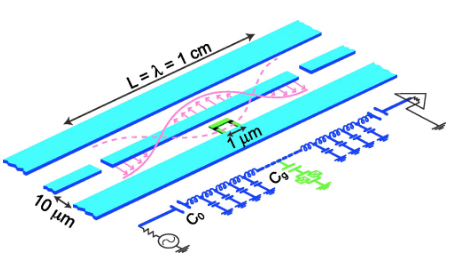
\includegraphics[width=0.309\textwidth]{QI10/a coplanar waveguide (CPW) resonator}
    \caption{a coplanar waveguide (CPW) resonator}
\end{figure}

The energy of a single mode with frequency $\omega_c$ is
\begin{align*}
    E_n=\left( n+\frac{1}{2} \right)\hbar\omega_c
\end{align*}

In the picture of quantum field, the electric field operator is $\vec{E}_c=\hat{\epsilon}E_{c0}(a+a^\dagger)$, where a is the photon annihilation operator and $\hat{\epsilon}$ the polarization direction.

Recall that the operators obey
\begin{itemize}\small
    \item $[a, a^\dagger]\equiv aa^\dagger -a^\dagger a=1$
    \item With $N=a^\dagger a, [a, N]=a$ and $[a^\dagger, N]=-a^\dagger$
\end{itemize}

We usually choose the eigenstates $\ket{n}$ of $N$ to be the basis.
\begin{itemize}\small
    \item $N\ket{n}=n\ket{n}$
    \item $a\ket{n}=\sqrt{n}\ket{n-1}$, where $\braket{n|n}=1$
\end{itemize}

In the number basis, it is rather easy to calculate matrix elements. The elementary ones are $\braket{n-1|a|n}=\sqrt{n}$ and $\braket{n+1|a^\dagger |n}=\sqrt{n+1}$. 

Alternatively, we can write
\begin{align*}
    a&= \sum_n\sqrt{n+1}\ket{n}\bra{n+1} \\
    a^\dagger &= \sum_n \sqrt{n+1}\ket{n+1}\bra{n}
\end{align*}

We can now associate the constant in the field operator
\begin{align*}
    E_{c0}\equiv \sqrt{\braket{0|E_c^2|0}}=\sqrt{\braket{0|E_{c0}a|1}\braket{1|E_{c0}a^\dagger|0}}
\end{align*}
with vacuum fluctuations (through virtual photon emission and reabsorption) in the vacuum $\ket{0}$. 

Meanwhile, the energy due to vacuum fluctuations is
\begin{align*}
    \frac{\hbar\omega}{2}=2V_c\left[ \frac{\epsilon_0\braket{0|E_c^2|0}}{2} \right]
\end{align*}
where $V_c$ is the volume of the cavity and the factor of 2 takes care of the coexisting magnetic field energy. So,
\begin{align*}
    E_{c0}=\sqrt{\braket{0|E_c^2|0}}=\sqrt{\frac{\hbar\omega_c}{2\epsilon_0 V_c}}
\end{align*}

One can conclude that a small cavity enhances quantum fluctuations of the electric field. 

\subsection{Coupling Between Atom and EM Field}
With the quantized field, we can establish a fully quantum-mechanical model to describe the interaction between qubits and photons.

The Jaynes-Cummings model has a Hamiltonian
\begin{align*}
    H_{JC}=-\underbrace{{\frac{1}{2}\hbar\omega_{01}\sigma_z}}_{H_{qbuit}} + \underbrace{\hbar \omega_c\left(a^\dagger a +\frac{1}{2}\right)}_{H_{field}} + \underbrace{\hbar g (a\sigma_+ + a^\dagger \sigma_-)}_{H_{int}}
\end{align*}
where $\sigma_\pm=\frac{\sigma_x \pm i\sigma_y}{2}$. Notice that $\sigma_+\ket{g}=\ket{e}, \sigma_-\ket{e}=\ket{g}$ and $\sigma_+\ket{e}=\sigma_-\ket{g}=0$. 

The quantum Hamiltonian arises from a coupling between the electric field $\vec{E}$ in a single-mode cavity and the dipole moment $\vec{p}$ of the artificial atom at position $\vec{R}$ given by
\begin{align*}
    U=-\vec{p}\cdot\vec{E}(\vec{R})
\end{align*}

This dipole moment connects the ground and excited state of the atom, and the interaction term reads
\begin{align*}
    H_{int}&=-\ket{e}\braket{e|\vec{p}\cdot\vec{E}(\vec{R})|g}\bra{g}+h.c.\\
    &=\hbar g (a+a^\dagger)\sigma_x
\end{align*}
where the vacuum Rabi coupling
\begin{align*}
    g=-\braket{e|\vec{p}\cdot \hat{\epsilon}|g}\frac{E_{c0}}{\hbar}
\end{align*}

The interaction can be rewritten as
\begin{align*}
    H_{int}&= \hbar g (a+a^\dagger)(\sigma_+ + \sigma_-)\\
    &=\hbar g (a\sigma_+ + a^\dagger \sigma_-)+\hbar g (a\sigma_- + a^\dagger \sigma_+)
\end{align*}

If the cavity mode is close in frequency to the qubit transition frequency, the first term is important because it nearly conserves the total energy. 

The second term mixing states that are far away from each other is often dropped in the so-called \textbf{rotating wave approximation}.

We arrive at the Jaynes-Cummings Hamiltonian, which may further include external driving and damping terms.

\subsubsection{Solving the JC Hamiltonian}
The Hilbert space is the tensor product of a harmonic oscillator and a qubit, whose basis vectors are
\begin{align*}
    \ket{0, g}, \ket{1, g}, \ket{2, g}, \cdots\\
    \ket{0, e}, \ket{1, e}, \ket{2, e}, \cdots
\end{align*}
where the first index is the number of photons and the second the qubit state $(g \equiv 0, e \equiv 1)$. (详细见 lab8)

The first two terms in $H_{JC}$ is already diagonal, i.e.,
\begin{align*}
    \braket{n, \sigma | H_{qubit}+H_{field} |m, \sigma'}=(\hbar \omega_{01}\sigma+n\hbar\omega_c)\delta_{nm}\delta_{\sigma\sigma'}
\end{align*}
up to an unimportant constant. 

\begin{figure}[!htb]
    \centering
    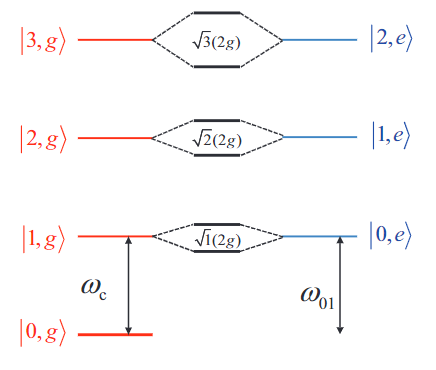
\includegraphics[width=0.309\textwidth]{QI10/a harmonic oscillator and a qubit}
    \caption{a harmonic oscillator and a qubit}
\end{figure}

To be exact, we need infinitely many basis states. However, when the temperature is low and when we are not interested in pumping in more than a few photons, we can truncate the Hilbert space to include just a few basis states (in the absence of qubit-cavity interaction). 

Let us consider the case where the detuning between the qubit and cavity frequencies
\begin{align*}
    \Delta\equiv \omega_{01}-\omega_c=0
\end{align*}
Photon and qubit excitations hybrid into the so-called polaritons.

In the case $\Delta = 0$, the two states $\ket{n + 1, g}$ and $\ket{n, e}$ are degenerate in the absence of interaction. 

The dipole coupling lift the degeneracy by introducing off-diagonal matrix elements (which are real)
\begin{align*}
    \braket{n+1, g|H_{int}|n,e}=\braket{n,e|H_{int}|n+1, g}=\sqrt{n+1}\hbar g
\end{align*}
In the truncated 2D subspace, the effective Hamiltonian is
\begin{align*}
    H'&=\begin{pmatrix}
        (n+1)\hbar\omega_c & \sqrt{n+1}\hbar g\\
        \sqrt{n+1}\hbar g & (n+1)\hbar\omega_c
    \end{pmatrix}\\
    &=(n+1)\hbar \omega_c I_{2\times 2}+\sqrt{n+1}\hbar g\sigma_x
\end{align*}
The energy eigenstates are coherent superpositions
\begin{align*}
    \ket{\Psi_\pm}=\frac{1}{\sqrt{2}}(\ket{n+1, g}\pm\ket{n,e})
\end{align*}
i.e., the bonding–anti-bonding combination of photon and qubit excitation, known as polaritons.

The corresponding energies are
\begin{align*}
    E_\pm =(n+1)\hbar\omega_c\pm\sqrt{n+1}\hbar g
\end{align*}
In this approximation, we have neglect the coupling of the levels to those with energy difference $2~\hbar\omega_c$ , due to the second term of the interaction (see Lab for explanation).

In the so-called dispersive regime, where $|\Delta|\gg g$, the truncated Hamiltonian becomes
\begin{align*}
    H'&=\begin{pmatrix}
        (n+1)\hbar\omega_c & \sqrt{n+1}\hbar g\\
        \sqrt{n+1}\hbar g & n\hbar\omega_c +\hbar\omega_{01}
    \end{pmatrix}\\
    &=\epsilon_n I_{2\times 2}+\sqrt{n+1}\hbar g \sigma_x - \frac{\hbar \Delta}{2}\sigma_z
\end{align*}
where 
\begin{align*}
    \epsilon_n=\left( n+\frac{1}{2} \right)\hbar\omega_c+\frac{1}{2}\hbar\omega_{01}
\end{align*}
One can verify that $H'$ reduces to the degenerate form when $\Delta\equiv \omega_{01}-\omega_c=0$

Up to a constant, the Hamiltonian represents a spin in a pseudo magnetic field $\vec{B}=\left( \sqrt{n+1}\hbar g, 0, \frac{\Delta}{2} \right)$. Just like in a Stern-Gerlach measurement, the eigenenergies can be obtained as
\begin{align*}
    E_\pm =\epsilon_n\pm |\vec{B}|=\epsilon_n\pm \frac{\hbar\Delta}{2}\sqrt{1+\frac{4g^2}{\Delta^2}(n+1)}
\end{align*}
In the dispersive limit $(|\Delta|\gg g)$ we can perform a Taylor series expansion
\begin{align*}
    E_\pm=\epsilon_n\pm \frac{\hbar \Delta}{2}\left[ 1+\frac{1}{2}\frac{4g^2}{\Delta^2}(n+1)+O\left(  \frac{g}{\Delta}^4 \right) \right]
\end{align*}
Comparing to the uncoupled system
\begin{align*}
    \Delta E_{n+1, g}&=-\hbar\frac{g^2}{\Delta}(n+1)=-\hbar\frac{g^2}{\Delta}\left[ (n+1)+\frac{1}{2} \right]+\hbar \frac{g^2}{\Delta}\\
    \Delta E_{n, g}&=\hbar\frac{g^2}{\Delta}(n+1)=\hbar\frac{g^2}{\Delta}\left( n+\frac{1}{2} \right)+\hbar \frac{g^2}{\Delta}
\end{align*}

The coupling introduces an effective potential, up to a constant
\begin{align*}
    V_{dispersive}=-\hbar \frac{g^2}{\Delta}\left[ a^\dagger a+\frac{1}{2} \right]\sigma_z
\end{align*}
in the limit of $g\rightarrow 0$. 

\begin{figure}[!htb]
    \centering
    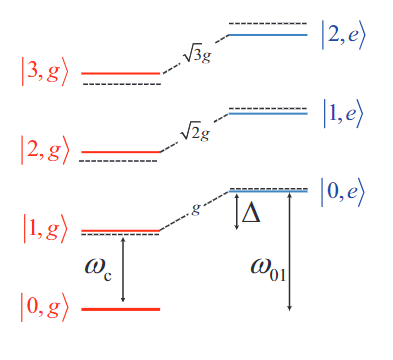
\includegraphics[width=0.309\textwidth]{QI10/the result of a second-order perturbation}
    \caption{the result of a second-order perturbation}
\end{figure}

This is result of a second-order perturbation. It can be interpreted as a shift in the cavity frequency which depends on the state of the qubit, thus can be measured without directly disturbing the qubit state. 

\subsection{Two Qubits Coupled Through a Cavity}
Two qubits connected to the same resonator can be coupled passively through its virtual excitations.

\begin{figure}[!htb]
    \centering
    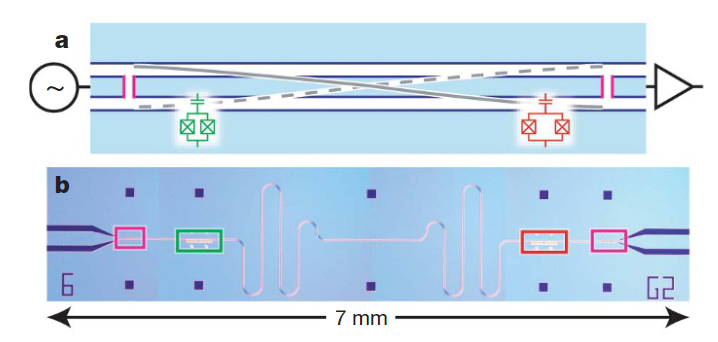
\includegraphics[width=0.309\textwidth]{QI10/Two Qubits Coupled Through a Cavity}
    \caption{Two Qubits Coupled Through a Cavity}
\end{figure}

The effective Hamiltonian for the resonator and two such qubits can be obtained as
\begin{align*}
    H_{12}^{eff}=&\left[ \hbar\omega_c\left( a^\dagger a +\frac{1}{2}\right) \right]_{field}-\left[ \frac{\hbar\omega_{01}}{2}(\sigma_{1z}+\sigma_{2z}) \right]_{qubits}\\
    &-\frac{\hbar g^2}{\Delta}\left( a^\dagger a+\frac{1}{2} \right)(\sigma_{1z}+\sigma_{2z})\\
    &-\frac{\hbar g^2}{\Delta}(\sigma_{1+}\sigma_{2-}+\sigma_{1-}\sigma_{2+})
\end{align*}

\begin{figure}[!htb]
    \centering
    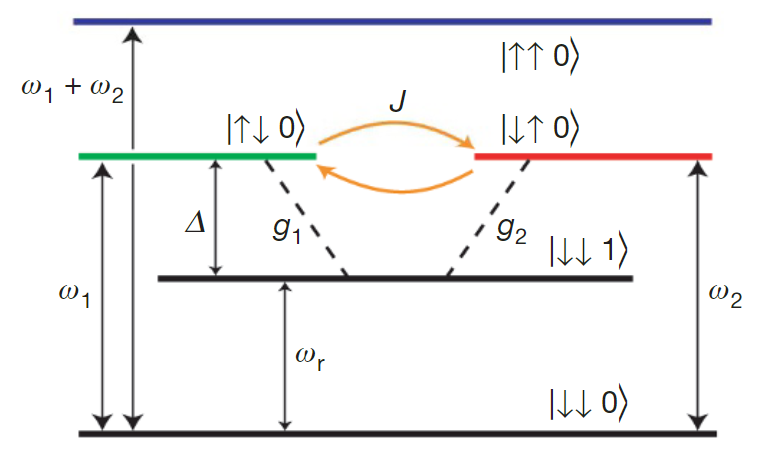
\includegraphics[width=0.309\textwidth]{QI10/the state of the resonator mode}
    \caption{ the state of the resonator mode}
\end{figure}

The qubits should be tuned in resonance with each other, but away from the resonator's frequency.

In the qubit subspace
\begin{align*}
    U(t)=&e^{i\frac{\hbar g^2}{\Delta}\left( a^\dagger a+\frac{1}{2} \right)(\sigma_{1z}+\sigma_{2z})}\\
    &\begin{pmatrix}
        1 & 0 & 0 & 0\\
        0 & \cos\frac{g^2}{\Delta}t & i\sin \frac{g^2}{\Delta}t & 0\\
        0 & i\sin \frac{g^2}{\Delta}t & \cos \frac{g^2}{\Delta}t& 0\\
        0 & 0 & 0 & 1
    \end{pmatrix}
\end{align*}
This does not change the state of the resonator mode. At $t=\frac{\pi |\Delta|}{4g^2}$, it corresponds to a $\sqrt{i SWAP}$ operation.


